\documentclass[xetex,mathserif,serif]{beamer}
\usepackage{polyglossia}
\setdefaultlanguage[babelshorthands=true]{russian}
\usepackage{minted}
\usepackage{tabu}

\useoutertheme{infolines}

\usepackage{fontspec}
\setmainfont{FreeSans}
\newfontfamily{\russianfonttt}{FreeSans}

\usepackage{textpos}
\setlength{\TPHorizModule}{1cm}
\setlength{\TPVertModule}{1cm}

\tabulinesep=1.2mm

\title[Шаблоны]{Лекция 8: Поведенческие шаблоны}
\author[Юрий Литвинов]{Юрий Литвинов\\\small{\textcolor{gray}{y.litvinov@spbu.ru}}}
\date{26.10.2021}

\newcommand{\DownArrow} {
    \hspace{2cm}\begin{LARGE}$\downarrow$\end{LARGE}
}

\newcommand{\attribution}[1] {
    \vspace{-5mm}\begin{flushright}\begin{scriptsize}\textcolor{gray}{\textcopyright\, #1}\end{scriptsize}\end{flushright}
}

\begin{document}

    \frame{\titlepage}

    \section{Паттерн ``Строитель''}

    \begin{frame}
        \frametitle{``Строитель'', мотивация}
        \framesubtitle{Конвертер текста}
        \begin{center}
            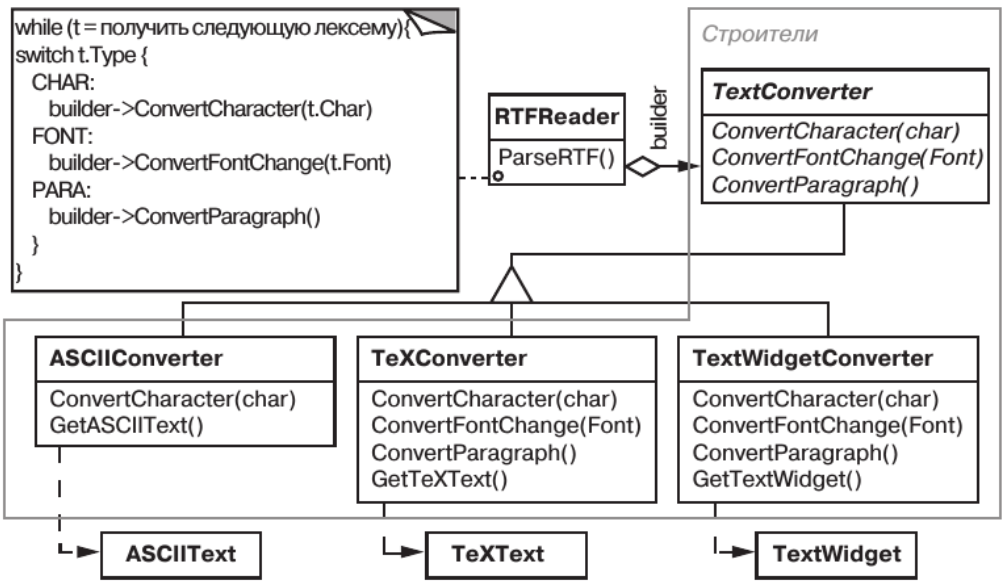
\includegraphics[width=0.8\textwidth]{textConverter.png}
        \end{center}
    \end{frame}

    \begin{frame}
        \frametitle{Патерн ``Строитель''}
        \framesubtitle{Builder}
        \begin{center}
            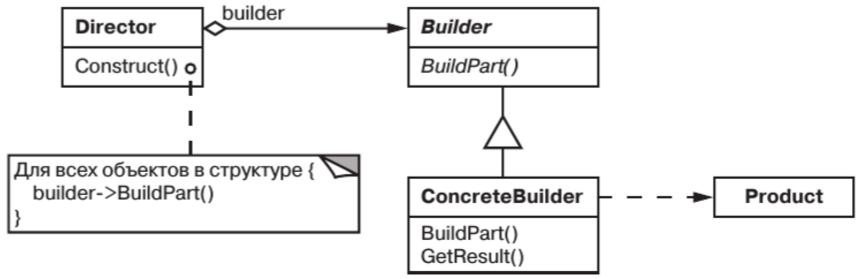
\includegraphics[width=0.85\textwidth]{builder.png}
        \end{center}
    \end{frame}
    
    \begin{frame}
        \frametitle{``Строитель'' (Builder), детали реализации}
        \begin{center}
            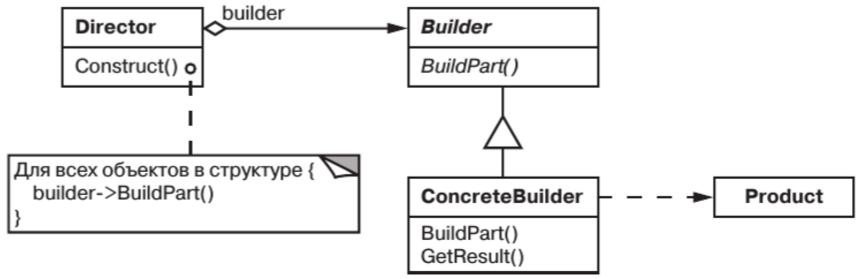
\includegraphics[width=0.7\textwidth]{builder.png}
        \end{center}
        \begin{itemize}
            \item Абстрактные и конкретные строители
            \begin{itemize}
                \item Достаточно общий интерфейс
            \end{itemize}
            \item Общий интерфейс для продуктов не требуется
            \begin{itemize}
                \item Клиент конфигурирует распорядителя конкретным строителем, он же и забирает результат
            \end{itemize}
            \item Пустые методы по умолчанию
        \end{itemize}
    \end{frame}

    \begin{frame}[fragile]
        \frametitle{``Строитель'', примеры}
        \begin{itemize}
            \item StringBuilder
            \item Guava, подсистема работы с графами
            \begin{minted}{java}
MutableNetwork<Webpage, Link> webSnapshot = 
        NetworkBuilder.directed()
    .allowsParallelEdges(true)
    .nodeOrder(ElementOrder.natural())
    .expectedNodeCount(100000)
    .expectedEdgeCount(1000000)
    .build();
            \end{minted}
        \end{itemize}
    \end{frame}

    \section{Паттерн ``Наблюдатель''}

    \begin{frame}
        \frametitle{Паттерн ``Наблюдатель'', мотивация}
        \begin{center}
            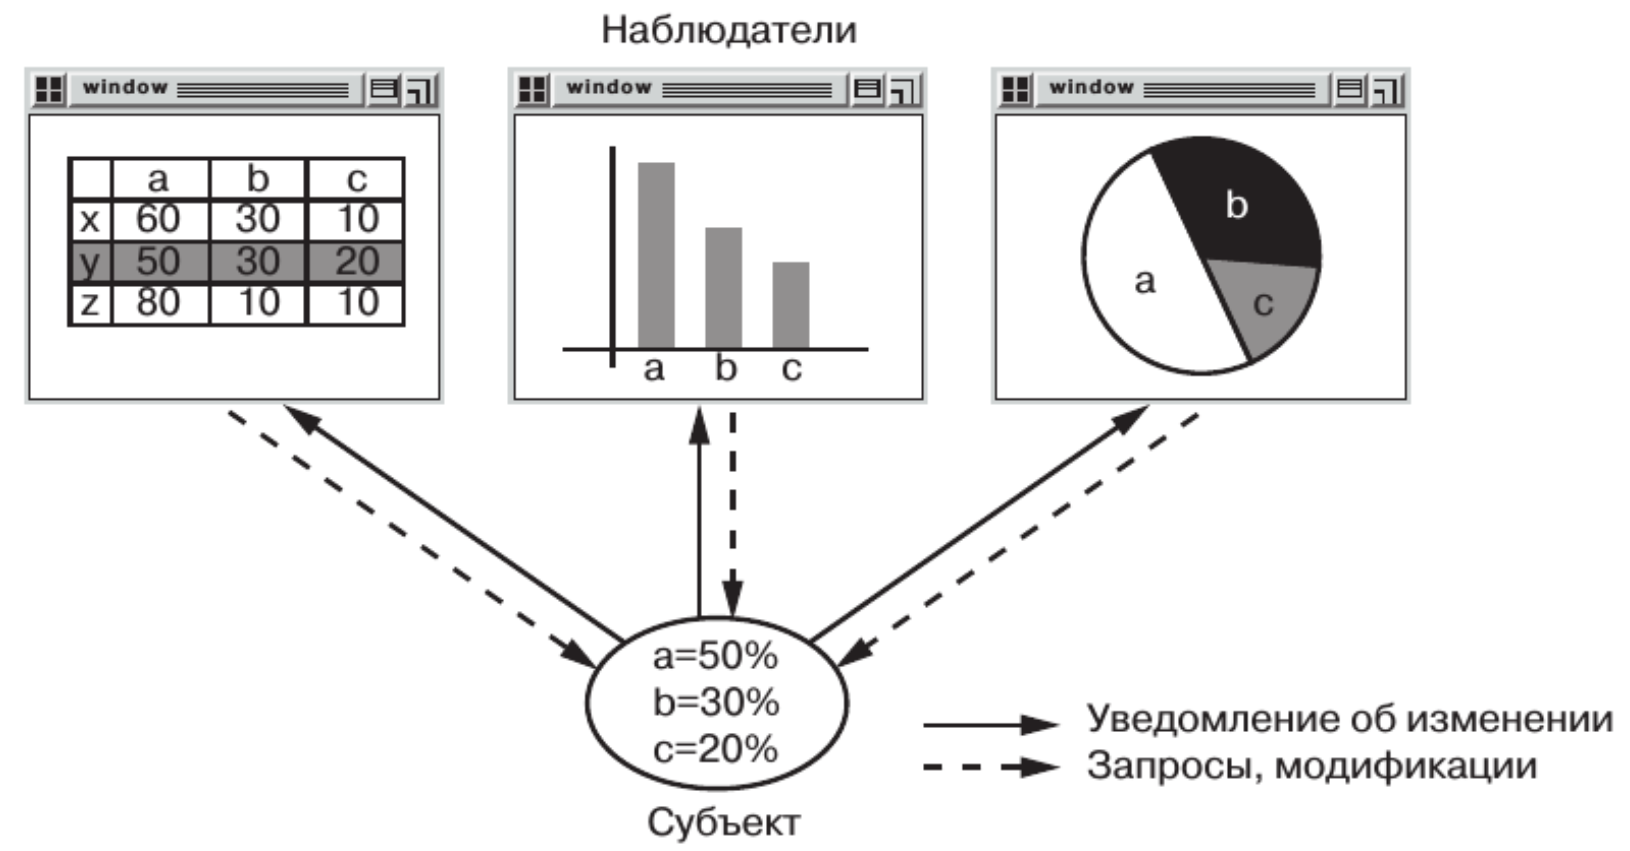
\includegraphics[width=0.9\textwidth]{observerExample.png}
        \end{center}
    \end{frame}

    \begin{frame}
        \frametitle{Паттерн ``Наблюдатель''}
        \begin{center}
            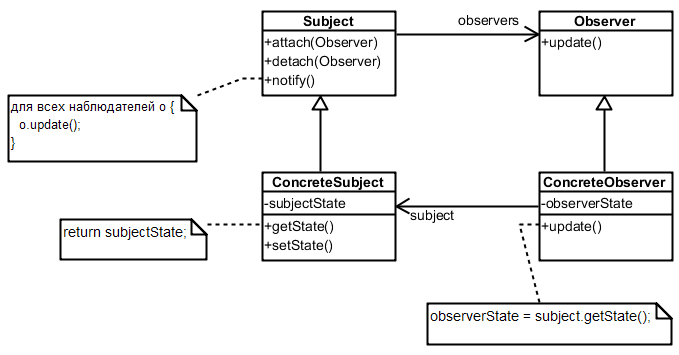
\includegraphics[width=0.75\textwidth]{observer.png}
        \end{center}
    \end{frame}

    \begin{frame}
        \frametitle{``Наблюдатель'' (Observer), детали реализации}
        \begin{itemize}
            \item Во многих языках поддержан ``из коробки'' (через механизм событий)
            \item Могут использоваться хеш-таблицы для отображения субъектов и наблюдателей
            \begin{itemize}
                \item Так делает WPF в .NET, есть даже языковая поддержка в C\#
            \end{itemize}
            \item Необходимость идентифицировать субъект
            \item Кто инициирует нотификацию
            \begin{itemize}
                \item Операции, модифицирующие субъект
                \item Клиент, после серии модификаций субъекта
            \end{itemize}
        \end{itemize}
    \end{frame}

    \begin{frame}
        \frametitle{``Наблюдатель'' (Observer), детали реализации (2)}
        \begin{itemize}
            \item Ссылки на субъектов и наблюдателей
            \begin{itemize}
                \item Простой способ организовать утечку памяти в C\# или грохнуть программу в C++
            \end{itemize}
            \item Консистентность субъекта при отправке нотификации
            \begin{itemize}
                \item Очевидно, но легко нарушить, вызвав метод предка в потомке
                \item ``Шаблонный метод''
                \item Документировать, кто когда какие события бросает
            \end{itemize}
            \item Передача сути изменений --- pull vs push
            \item Фильтрация по типам событий
            \item Менеджер изменений (``Посредник'')
        \end{itemize}
    \end{frame}

    \section{Паттерн ``Шаблонный метод''}

    \begin{frame}
        \frametitle{Паттерн ``Шаблонный метод'', мотивация}
        \begin{center}
            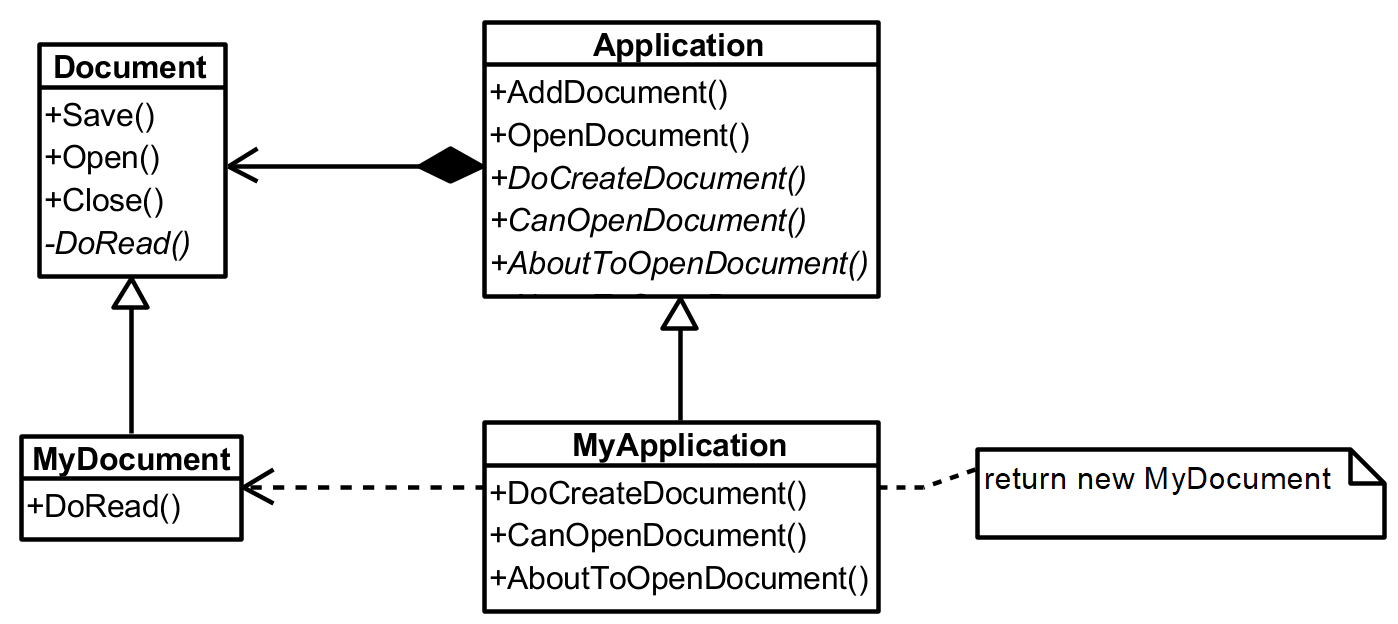
\includegraphics[width=0.7\textwidth]{templateMethodMotivation.png}
        \end{center}
        \begin{itemize}
            \item Алгоритм, общий для всех потомков
            \item Детали реализации операций --- в потомках
            \item Задание точек расширения
        \end{itemize}
    \end{frame}

    \begin{frame}[fragile]
        \frametitle{Шаблонный метод, пример}
        \begin{minted}{cpp}
void Application::OpenDocument(const char* name) {
   if (!CanOpenDocument(name)) {
       return;
   }

   Document* doc = DoCreateDocument();
  
   if (doc) {
       _docs->AddDocument(doc);
       AboutToOpenDocument(doc);
       doc->Open();
       doc->DoRead();
   }
}
        \end{minted}
    \end{frame}

    \begin{frame}
        \frametitle{``Шаблонный метод'' (Template Method), детали реализации}
        \begin{columns}
            \begin{column}{0.5\textwidth}
                \begin{itemize}
                    \item Сам шаблонный метод, как правило, невиртуальный
                    \item Лучше использовать соглашения об именовании, например, называть операции с Do
                \end{itemize}
            \end{column}
            \begin{column}{0.4\textwidth}
                \begin{center}
                    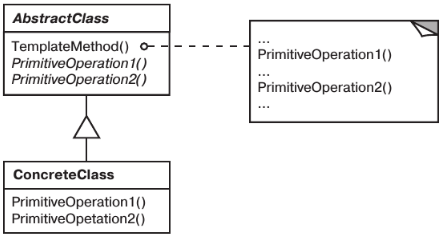
\includegraphics[width=\textwidth]{templateMethod.png}
                \end{center}
            \end{column}
        \end{columns}
        \begin{itemize}
            \item Примитивные операции могут быть виртуальными или чисто виртуальными
            \begin{itemize}
                \item Лучше их делать protected
                \item Чем их меньше, тем лучше
            \end{itemize}
        \end{itemize}
    \end{frame}

    \section{Паттерн ``Посредник''}

    \begin{frame}
        \frametitle{``Посредник'' (Mediator), мотивация}
        \begin{columns}
            \begin{column}{0.6\textwidth}
                \begin{itemize}
                    \item Большое количество связей между объектами
                    \item Объекты знают слишком много
                    \item Снижается переиспользуемость
                \end{itemize}
            \end{column}
            \begin{column}{0.4\textwidth}
                \begin{center}
                    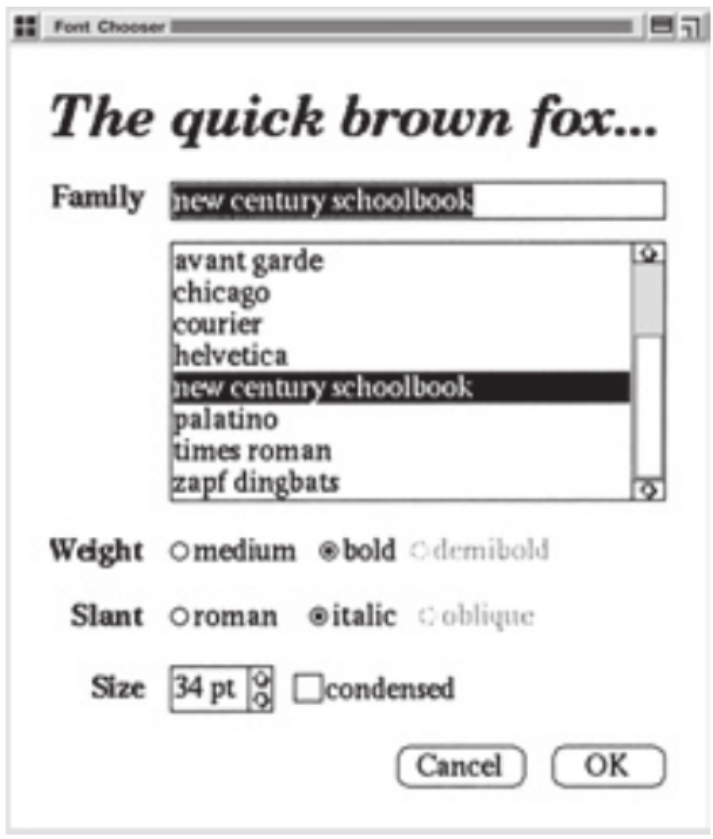
\includegraphics[width=0.7\textwidth]{mediatorMotivation.png}
                \end{center}
            \end{column}
        \end{columns}
    \end{frame}

    \begin{frame}
        \frametitle{Решение: централизация}
        \begin{center}
            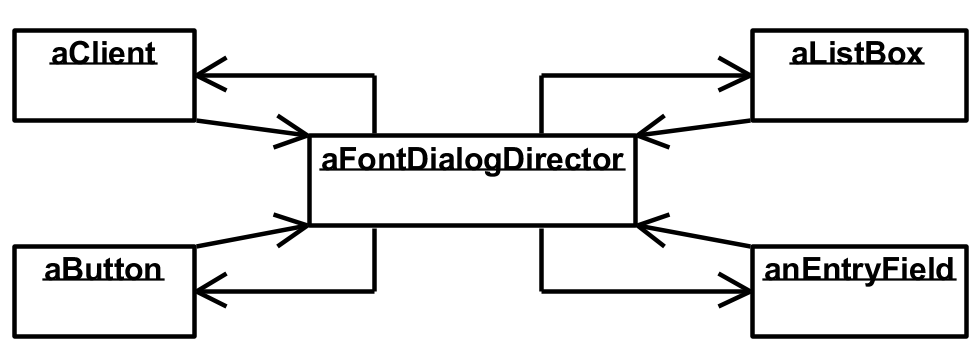
\includegraphics[width=0.5\textwidth]{mediatorObjectsDiagram.png}
        \end{center}
        \vspace{0.5cm}
        \begin{center}
            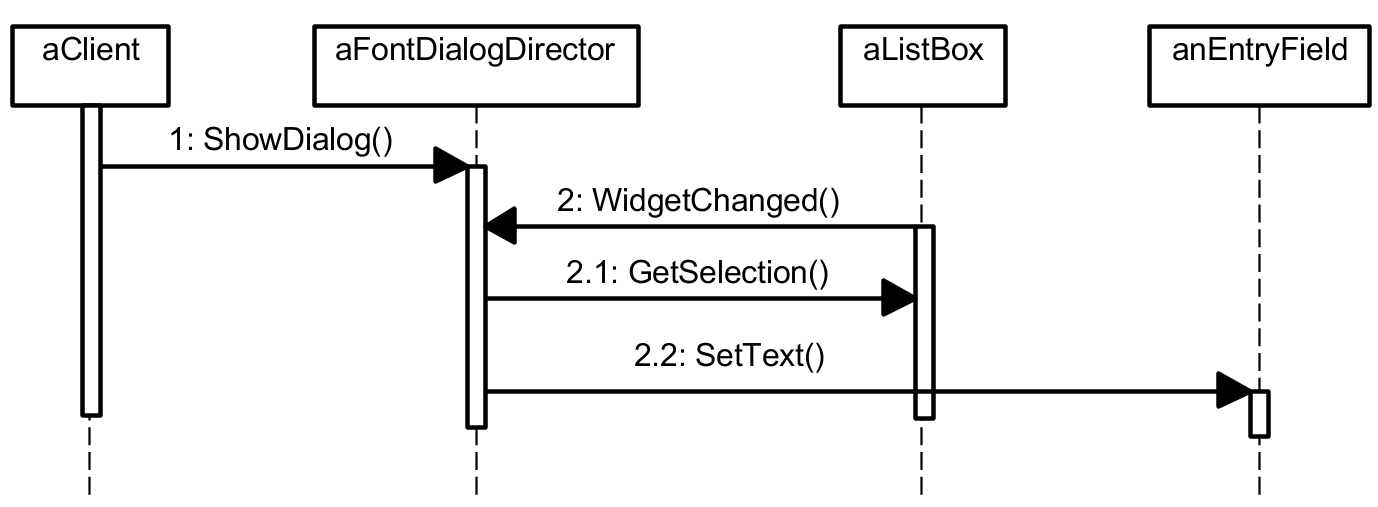
\includegraphics[width=0.8\textwidth]{mediatorSequence.png}
        \end{center}
    \end{frame}

    \begin{frame}
        \frametitle{Что получилось}
        \begin{center}
            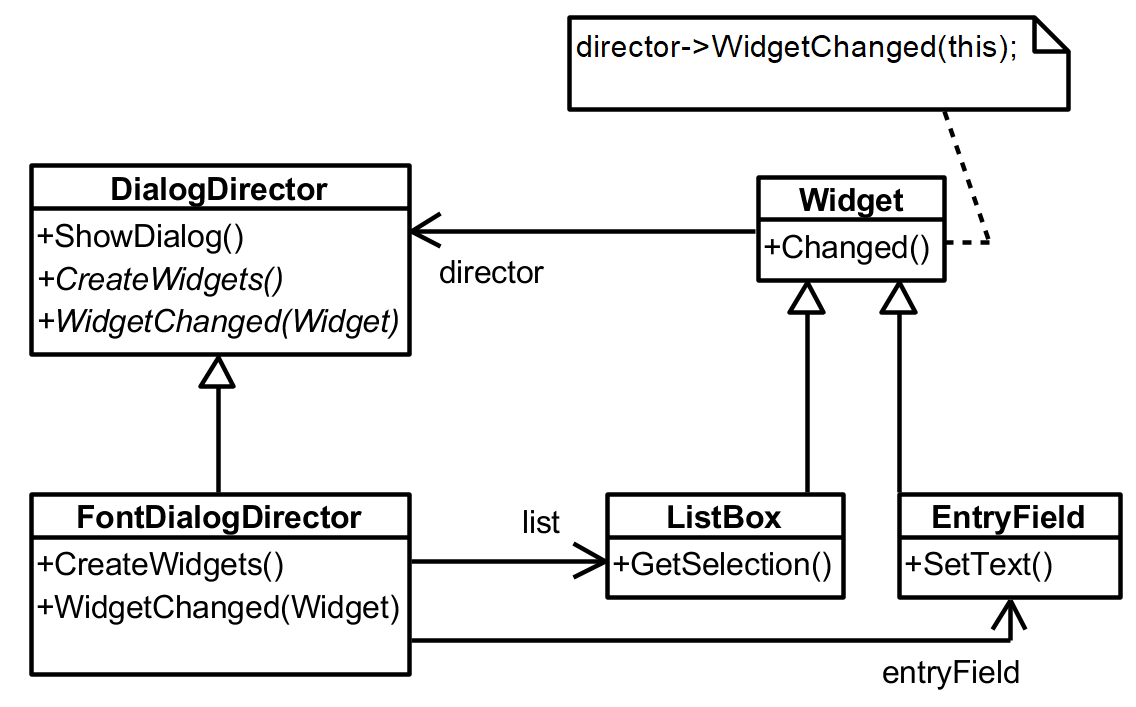
\includegraphics[width=0.7\textwidth]{mediatorStaticStructure.png}
        \end{center}
    \end{frame}

    \begin{frame}
        \frametitle{``Посредник'' (Mediator), детали реализации}
        \begin{columns}
            \begin{column}{0.5\textwidth}
                \begin{itemize}
                    \item Абстрактный класс ``Mediator'' часто не нужен
                    \item Паттерн ``Наблюдатель'': медиатор подписывается на события в коллегах
                    \item Наоборот: коллеги вызывают методы медиатора
                \end{itemize}
            \end{column}
            \begin{column}{0.5\textwidth}
                \begin{center}
                    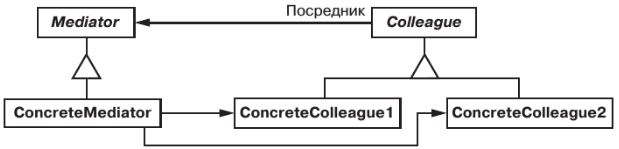
\includegraphics[width=\textwidth]{mediatorClasses.png}
                    \vspace{1cm}
                    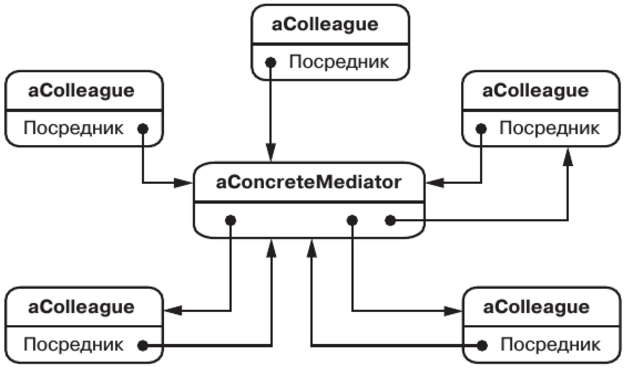
\includegraphics[width=\textwidth]{mediatorObjects.png}
                \end{center}
            \end{column}
        \end{columns}
    \end{frame}

    \begin{frame}
        \frametitle{Посредник, достоинства и недостатки}
        \begin{itemize}
            \item Устраняет связанность между классами-коллегами
            \item Повышает переиспользуемость классов-коллег
            \item Упрощает протоколы взаимодействия объектов
            \item Абстрагирует способ кооперирования объектов
            \item Централизует управление (потенциальный God Object!)
        \end{itemize}
    \end{frame}

    \section{Паттерн ``Команда''}

    \begin{frame}
        \frametitle{Паттерн ``Команда'', мотивация}
        \begin{itemize}
            \item Хотим отделить инициацию запроса от его исполнения
            \item Хотим, чтобы тот, кто ``активирует'' запрос, не знал, как он исполняется
            \item При этом хотим, чтобы тот, кто знает, когда исполнится запрос, не знал, когда он будет активирован
            \item Но зачем?
            \begin{itemize}
                \item Команды меню приложения
                \item Палитры инструментов
                \item ...
            \end{itemize}
            \item ``Просто вызвать действие'' не получится, вызов функции жёстко свяжет инициатора и исполнителя
        \end{itemize}
    \end{frame}

    \begin{frame}
        \frametitle{Решение: обернём действие в объект}
        \begin{center}
            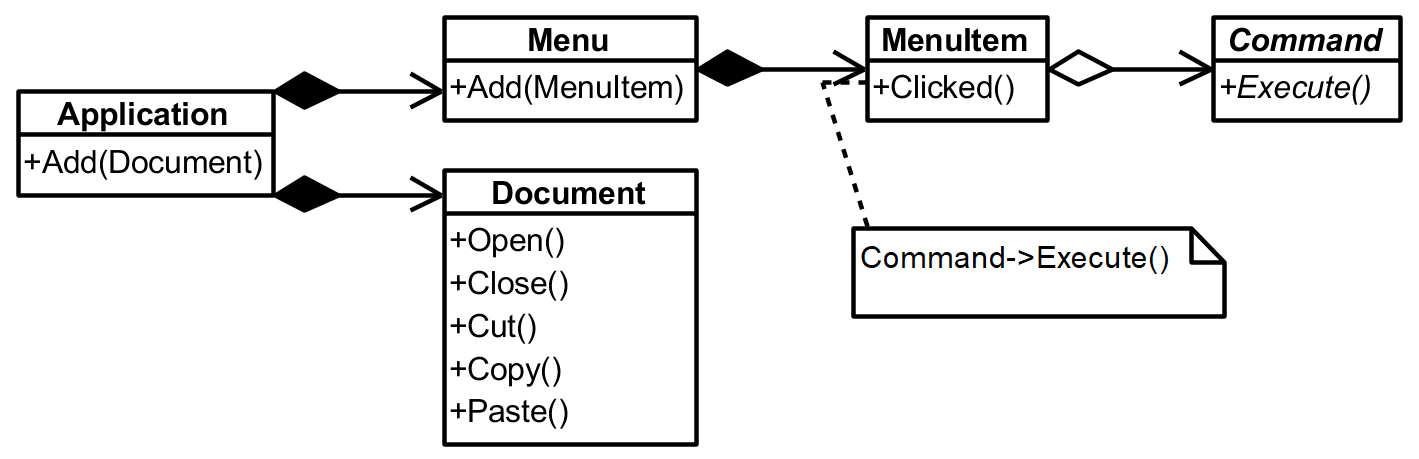
\includegraphics[width=0.9\textwidth]{commandExample.png}
        \end{center}
    \end{frame}

    \begin{frame}
        \frametitle{Команда вставки}
        \begin{center}
            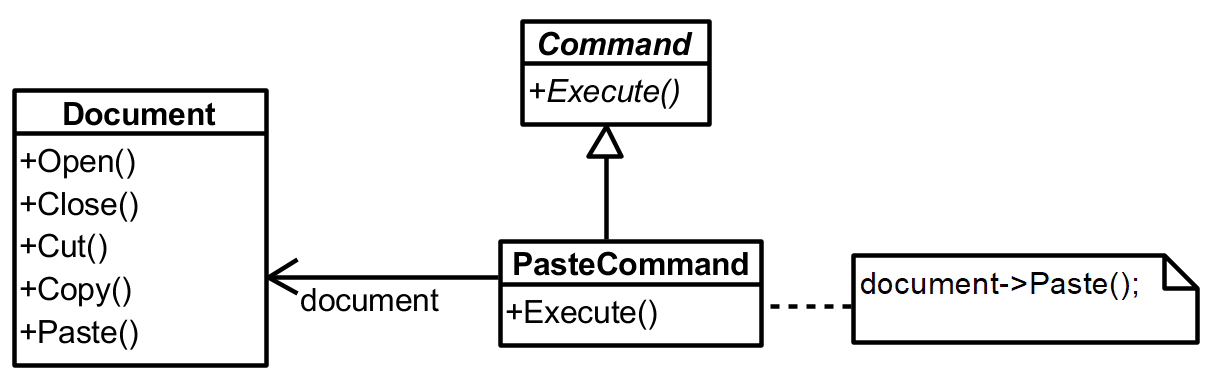
\includegraphics[width=0.75\textwidth]{pasteCommand.png}
        \end{center}
    \end{frame}

    \begin{frame}
        \frametitle{Команда открытия документа}
        \begin{center}
            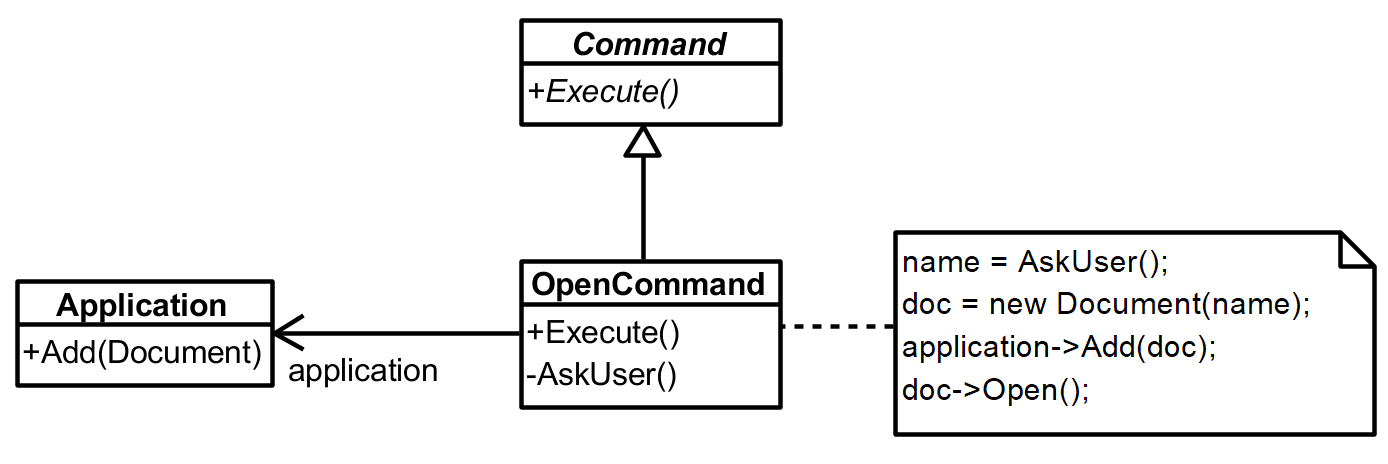
\includegraphics[width=0.75\textwidth]{openDocumentCommand.png}
        \end{center}
    \end{frame}

    \begin{frame}
        \frametitle{Составная команда}
        \begin{center}
            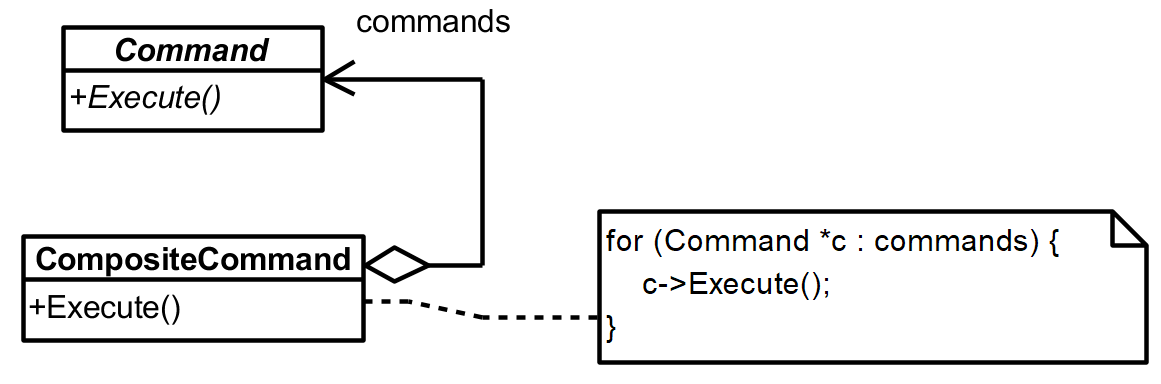
\includegraphics[width=0.75\textwidth]{compositeCommand.png}
        \end{center}
    \end{frame}

    \begin{frame}
        \frametitle{Паттерн ``Команда''}
        \begin{center}
            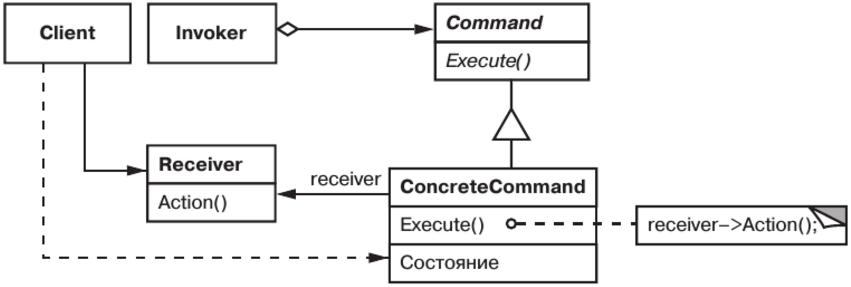
\includegraphics[width=0.9\textwidth]{command.png}
        \end{center}
    \end{frame}

    \begin{frame}
        \frametitle{Взаимодействие объектов}
        \begin{center}
            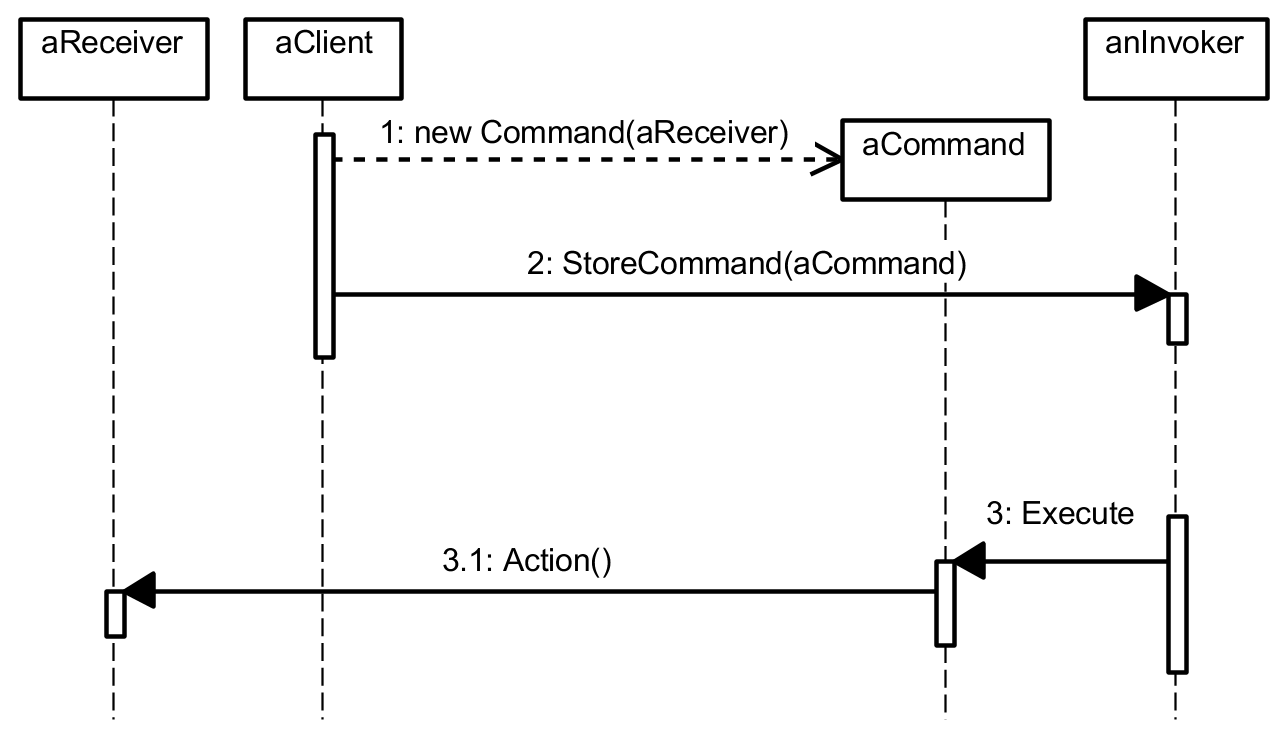
\includegraphics[width=0.9\textwidth]{commandSequence.png}
        \end{center}
    \end{frame}

    \begin{frame}
        \frametitle{Команда, применимость}
        \begin{itemize}
            \item Параметризовать объекты выполняемым действием
            \item Определять, ставить в очередь и выполнять запросы в разное время
            \item Поддержать отмену операций
            \item Структурировать систему на основе высокоуровневых операций, построенных из примитивных
            \item Поддержать протоколирование изменений
        \end{itemize}
    \end{frame}

    \begin{frame}
        \frametitle{``Команда'' (Command), детали реализации}
        \begin{itemize}
            \item Насколько ``умной'' должна быть команда
            \item Отмена и повторение операций --- тоже от хранения всего состояния в команде до ``вычислимого'' отката
            \begin{itemize}
                \item Undo-стек и Redo-стек
                \item Может потребоваться копировать команды
                \item ``Искусственные'' команды
                \item Композитные команды
            \end{itemize}
            \item Паттерн ``Хранитель'' для избежания ошибок восстановления
        \end{itemize}
    \end{frame}

    \begin{frame}[fragile]
        \frametitle{``Команда'', пример}
        \begin{itemize}
            \item Qt, класс QAction:
            \begin{minted}{c++}
const QIcon openIcon = QIcon(":/images/open.png");
QAction *openAct = new QAction(openIcon, tr("&Open..."), this);

openAct->setShortcuts(QKeySequence::Open);
openAct->setStatusTip(tr("Open an existing file"));

connect(openAct, &QAction::triggered, this, &MainWindow::open);

fileMenu->addAction(openAct);
fileToolBar->addAction(openAct);
            \end{minted}
        \end{itemize}
\end{frame}

    \section{Паттерн ``Цепочка ответственности''}

    \begin{frame}
        \frametitle{Паттерн ``Цепочка ответственности'', мотивация}
        \begin{center}
            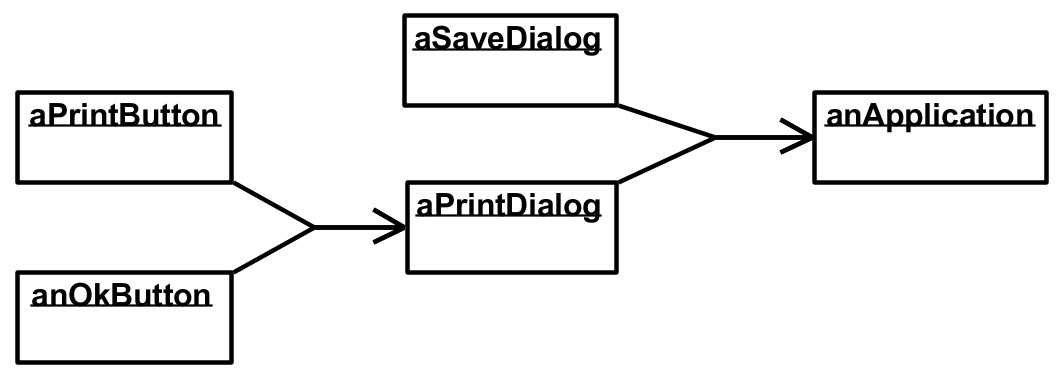
\includegraphics[width=0.7\textwidth]{chainOfResponsibilityExample.png}
        \end{center}
        \begin{itemize}
            \item Организация контекстной справки
            \item Если у элемента справки нет, запрос передаётся контейнеру
            \item Заранее неизвестно, кто в итоге обработает запрос
        \end{itemize}
    \end{frame}

    \begin{frame}
        \frametitle{Как это выглядит на диаграмме классов}
        \begin{center}
            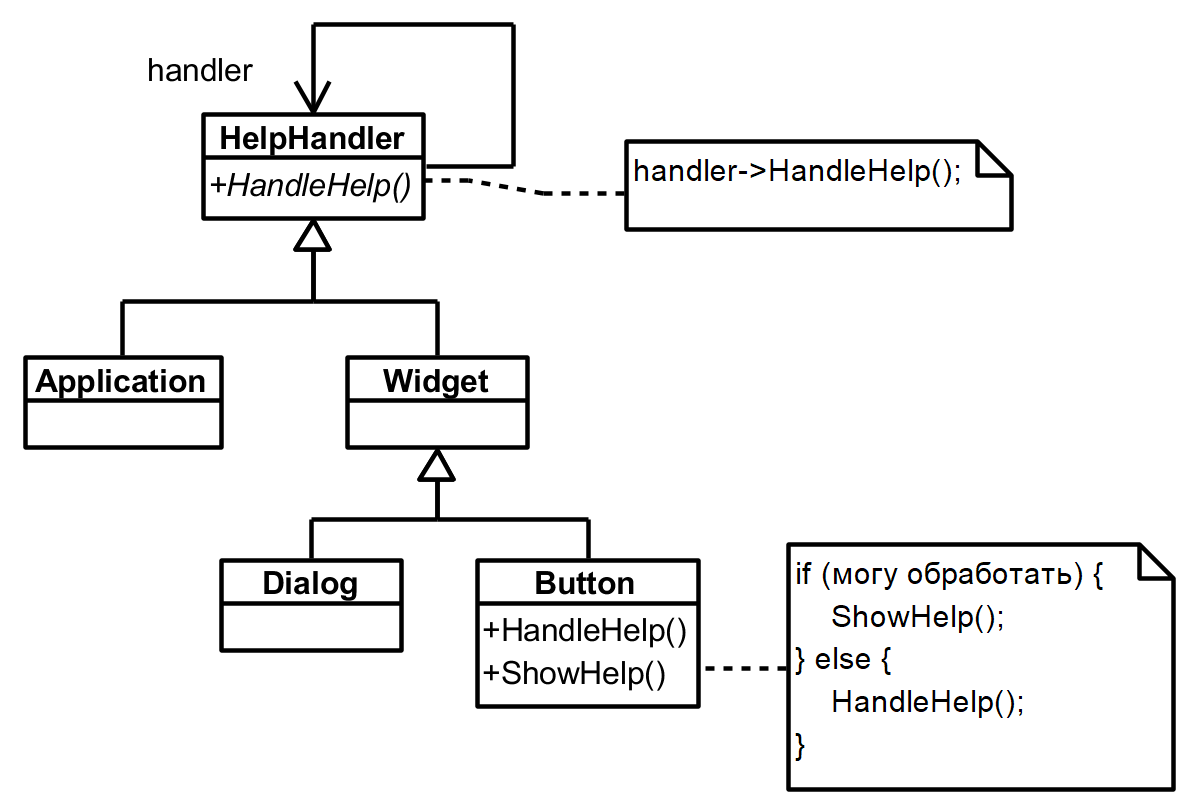
\includegraphics[width=0.8\textwidth]{chainOfResponsibilityExampleClasses.png}
        \end{center}
    \end{frame}

    \begin{frame}
        \frametitle{``Цепочка ответственности'' (Chain of Responsibility), детали реализации}
        \begin{columns}
            \begin{column}{0.5\textwidth}
                \begin{itemize}
                    \item Необязательно реализовывать связи в цепочке специально
                    \begin{itemize}
                        \item На самом деле, чаще используются существующие связи
                    \end{itemize}
                \end{itemize}
            \end{column}
            \begin{column}{0.5\textwidth}
                \begin{center}
                    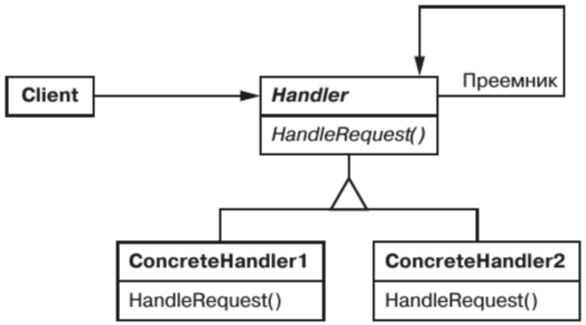
\includegraphics[width=\textwidth]{chainOfResponsibility.png}
                \end{center}
            \end{column}
        \end{columns}
        \begin{itemize}
            \item По умолчанию в Handler передавать запрос дальше (если ссылки на преемника всё-таки есть)
            \item Если возможных запросов несколько, их надо как-то различать
            \begin{itemize}
                \item Явно вызывать методы --- нерасширяемо
                \item Использовать объекты-запросы
            \end{itemize}
        \end{itemize}
    \end{frame}

    \begin{frame}
        \frametitle{``Цепочка ответственности'', плюсы и минусы}
        \begin{itemize}
            \item Ослабление связанности
            \item Дополнительная гибкость при распределении обязанностей
            \item Получение не гарантировано
        \end{itemize}
        Когда использовать:
        \begin{itemize}
            \item Есть более одного объекта-обработчика запросов
            \item Конечный обработчик неизвестен и должен быть найден автоматически
            \item Хотим отправить запрос нескольким объектам
            \item Обработчики могут задаваться динамически
        \end{itemize}
    \end{frame}

    \begin{frame}[fragile]
        \frametitle{``Цепочка ответственности'', примеры}
        \begin{itemize}
            \item Распространение исключений
            \item Распространение событий в оконных библиотеках:
            \begin{minted}{c++}
void MyCheckBox::mousePressEvent(QMouseEvent *event)
{
    if (event->button() == Qt::LeftButton) {
        // handle left mouse button here
    } else {
        // pass on other buttons to base class
        QCheckBox::mousePressEvent(event);
    }
}
            \end{minted}
        \end{itemize}
    \end{frame}

    \section{Паттерн ``Состояние''}

    \begin{frame}
        \frametitle{Паттерн ``Состояние'', мотивация}
        \begin{center}
            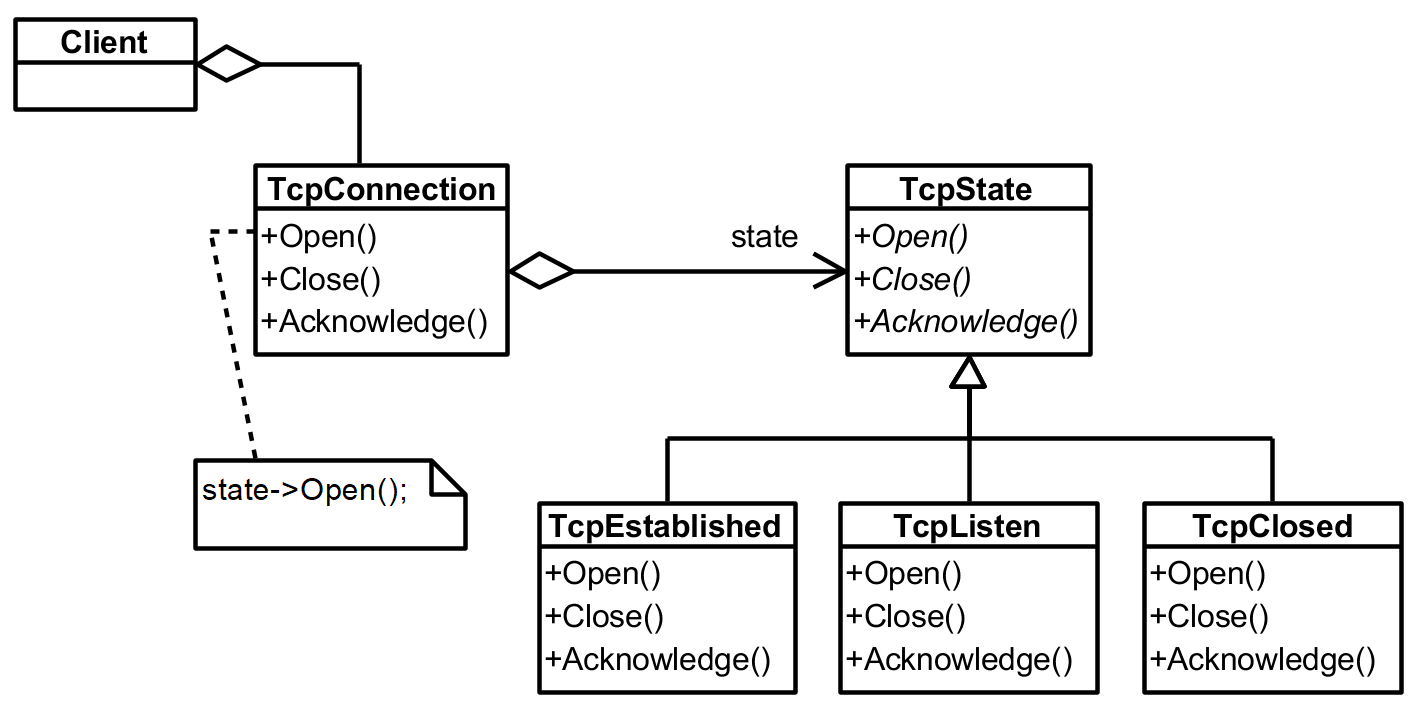
\includegraphics[width=0.85\textwidth]{stateExample.png}
        \end{center}
    \end{frame}

    \begin{frame}
        \frametitle{Паттерн ``Состояние''}
        \begin{center}
            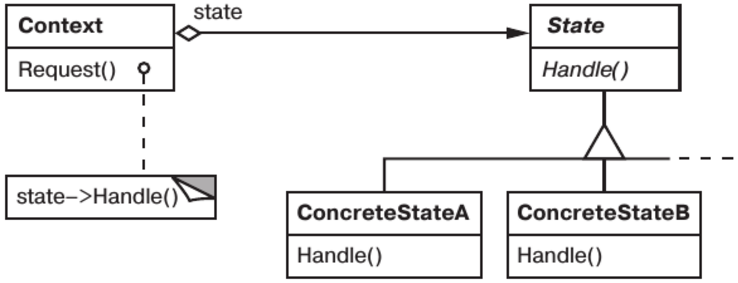
\includegraphics[width=0.75\textwidth]{state.png}
        \end{center}
    \end{frame}

    \begin{frame}
        \frametitle{``Состояние'' (State), детали реализации}
        \begin{itemize}
            \item Переходы между состояниями --- в Context или в State?
            \item Таблица переходов
            \begin{itemize}
                \item Трудно добавить действия по переходу
            \end{itemize}
            \item Создание и уничтожение состояний
            \begin{itemize}
                \item Создать раз и навсегда
                \item Создавать и удалять при переходах
            \end{itemize}
        \end{itemize}
    \end{frame}

    \begin{frame}
        \frametitle{``Состояние'' результаты}
        \begin{itemize}
            \item Локализует зависящее от состояния поведение
            \item Делает явными переходы между состояниями
            \item Объекты состояния можно разделять
        \end{itemize}
        Когда применять:
        \begin{itemize}
            \item Поведение объекта зависит от его состояния и должно изменяться во время выполнения
            \item Обилие условных операторов, в которых выбор ветви зависит от состояния
        \end{itemize}
    \end{frame}

    \section{Паттерн ``Посетитель''}

    \begin{frame}
        \frametitle{Паттерн ``Посетитель'', мотивация}
        \begin{center}
            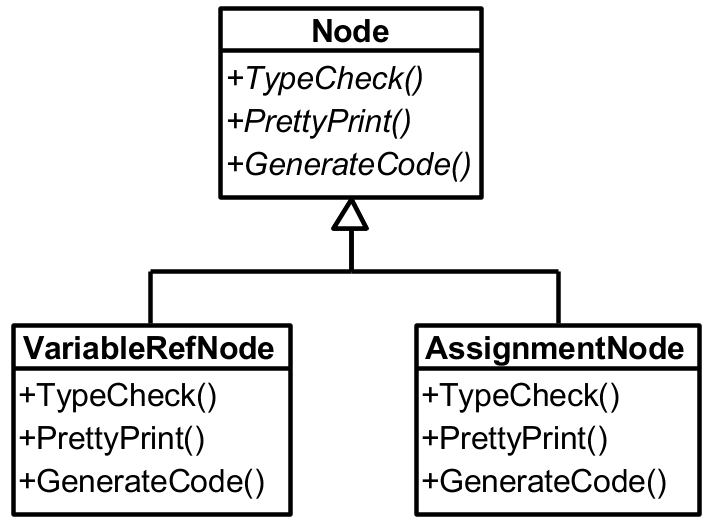
\includegraphics[width=0.4\textwidth]{visitorExample.png}
        \end{center}
        \begin{itemize}
            \item Синтаксическое дерево
            \item Много разных типов узлов
            \item Много разных операций, которые над ними можно выполнять
        \end{itemize}
    \end{frame}

    \begin{frame}
        \frametitle{Паттерн ``Посетитель'', решение}
        \begin{center}
            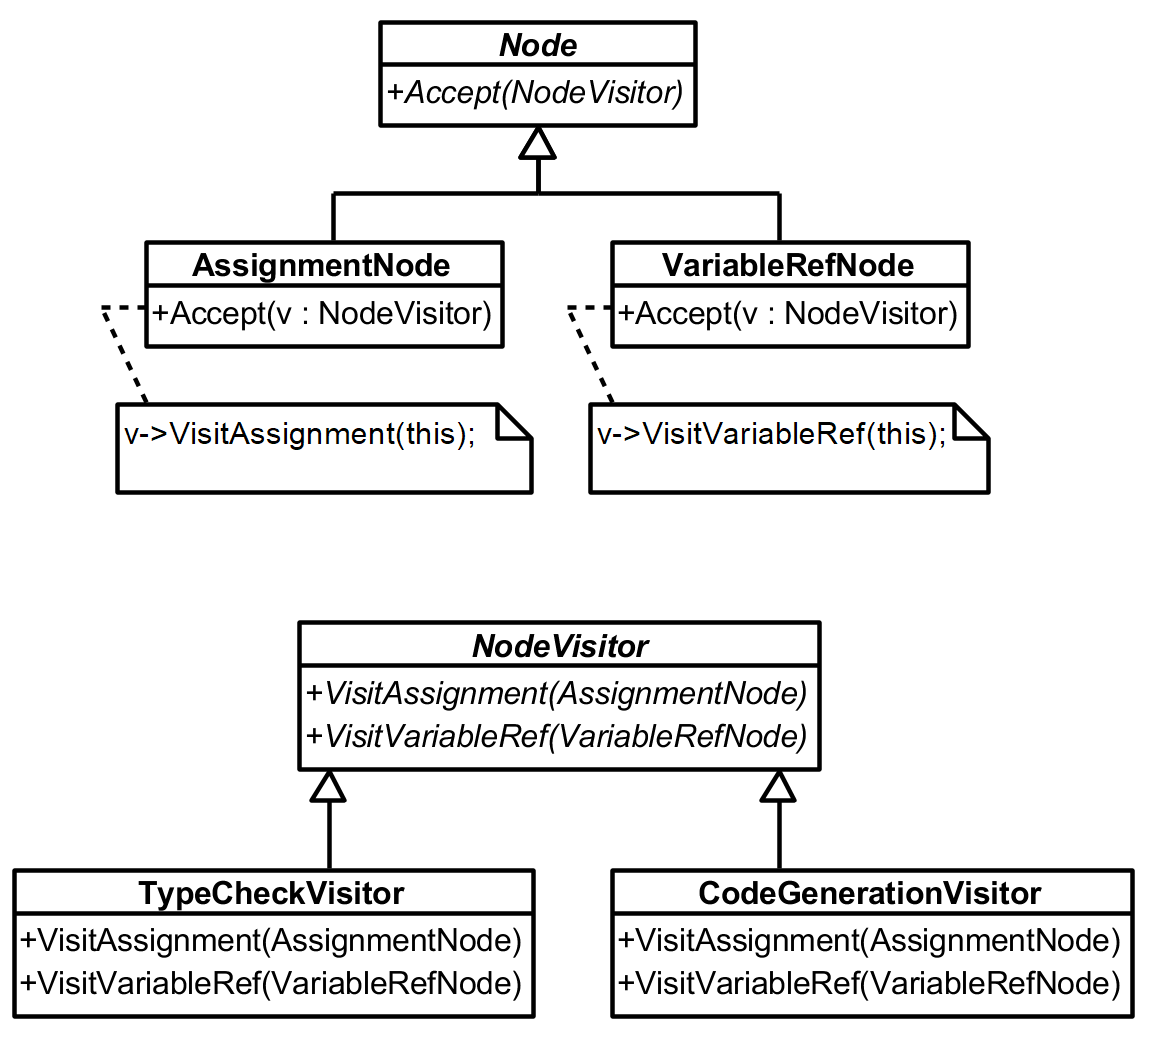
\includegraphics[width=0.7\textwidth]{visitorExampleSolution.png}
        \end{center}
    \end{frame}

    \begin{frame}
        \frametitle{Паттерн ``Посетитель''}
        \begin{center}
            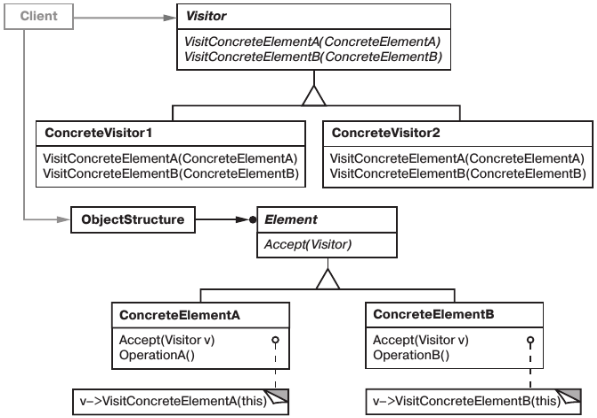
\includegraphics[width=0.75\textwidth]{visitor.png}
        \end{center}
    \end{frame}

    \begin{frame}
        \frametitle{Двойная диспетчеризация}
        \begin{center}
            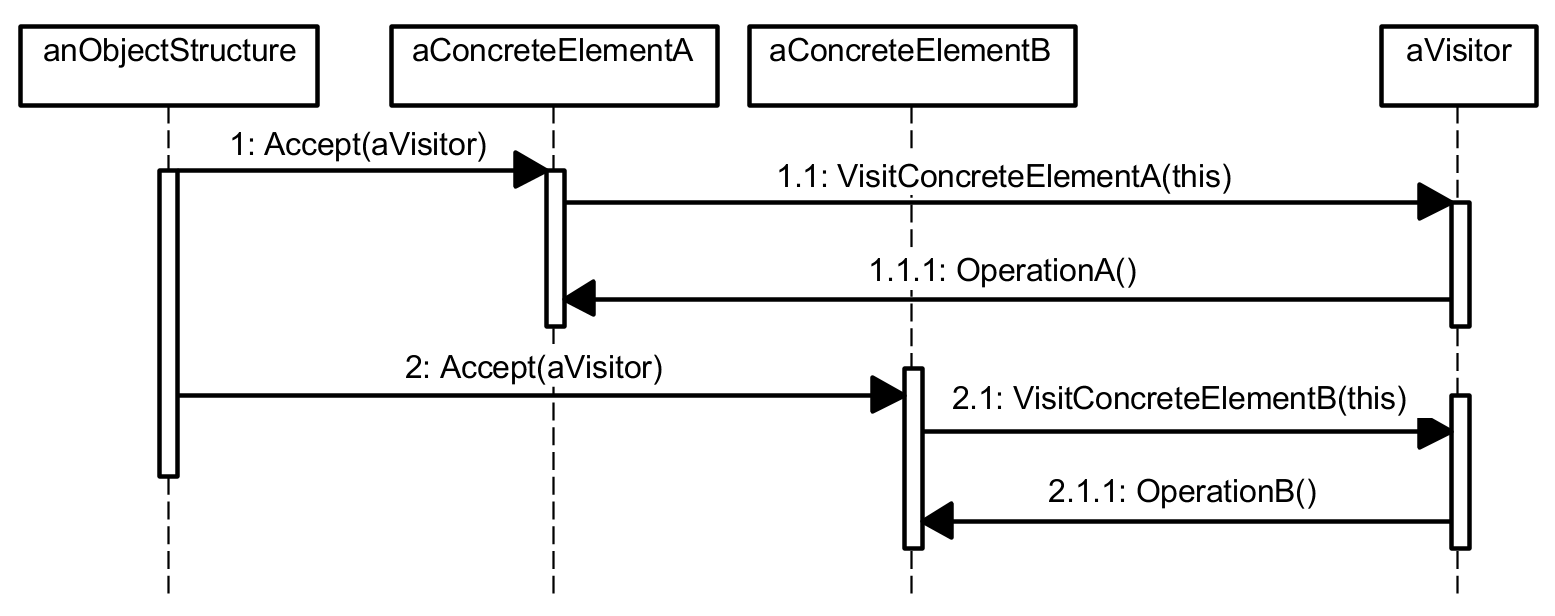
\includegraphics[width=0.9\textwidth]{doubleDispatching.png}
        \end{center}
    \end{frame}

    \begin{frame}
        \frametitle{``Посетитель'' (Visitor), детали реализации}
        \begin{itemize}
            \item Использовать перегрузку методов Visit(...)
            \item Чаще всего сама коллекция отвечает за обход, но может каждый элемент коллекции отдельно
            \item Может даже сам Visitor, если обход зависит от результата операции
            \item Аккумулирование состояния
            \item Несколько нарушает инкапсуляцию
            \item Просто добавлять новые операции, но сложно добавлять новые классы
        \end{itemize}
    \end{frame}

    \section{Паттерн ``Хранитель''}

    \begin{frame}
        \frametitle{Паттерн ``Хранитель'', мотивация}
        \begin{center}
            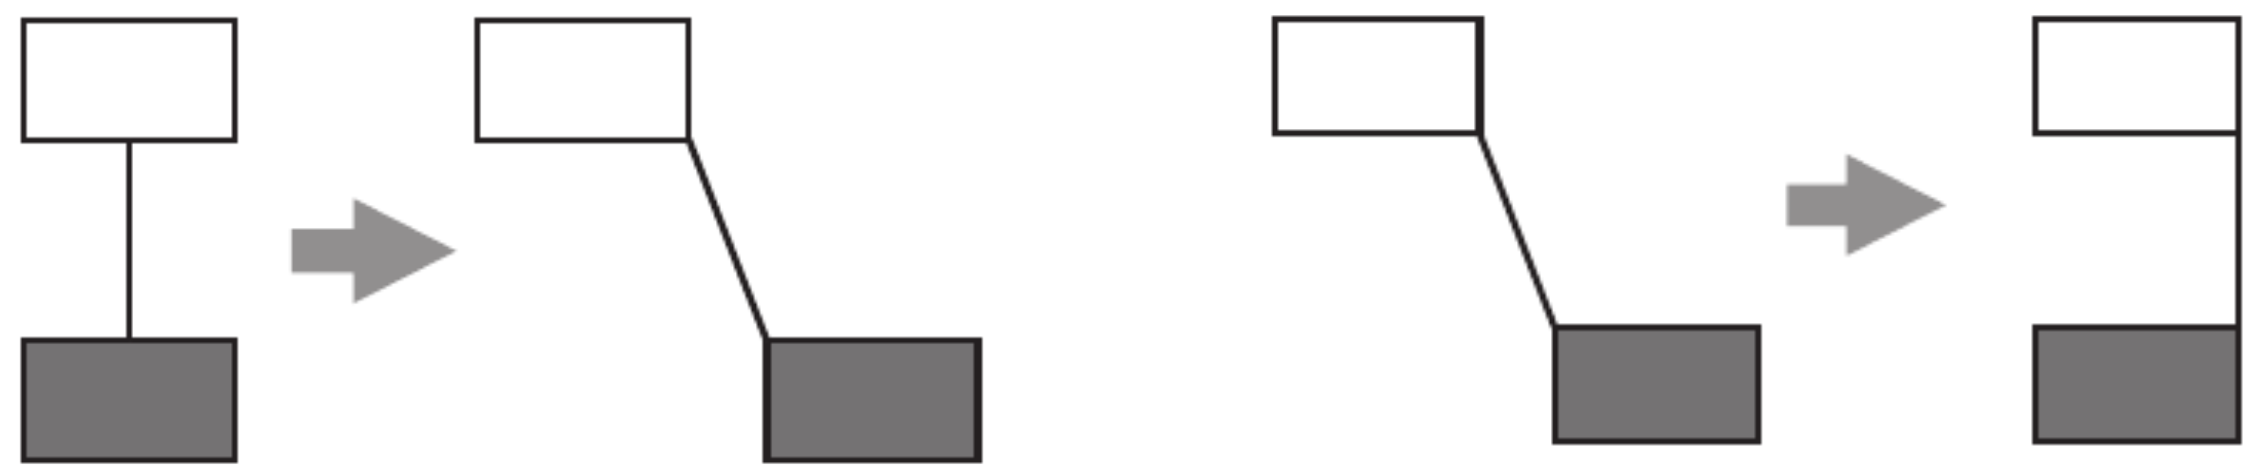
\includegraphics[width=0.9\textwidth]{mementoMotivation.png}
        \end{center}
        \begin{itemize}
            \item Хотим уметь фиксировать внутреннее состояние объектов
            \item И восстанавливать его при необходимости
            \item Не раскрывая внутреннего устройства объектов кому не надо
        \end{itemize}
    \end{frame}

    \begin{frame}
        \frametitle{Паттерн ``Хранитель''}
        \begin{center}
            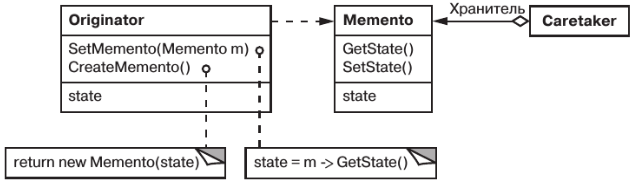
\includegraphics[width=0.7\textwidth]{memento.png}
        \end{center}
    \end{frame}

    \begin{frame}
        \frametitle{``Хранитель'' (Memento), детали реализации}
        \begin{itemize}
            \item Два интерфейса: ``широкий'' для хозяев и ``узкий'' для остальных объектов
            \begin{itemize}
                \item Требуется языковая поддержка
            \end{itemize}
            \item Можно хранить только дельты состояний
        \end{itemize}
    \end{frame}

    \section{Паттерн ``Интерпретатор''}

    \begin{frame}
        \frametitle{``Интерпретатор'' (Interpreter)}
        Определяет представление грамматики и интерпретатор для заданного языка.
        \begin{center}
            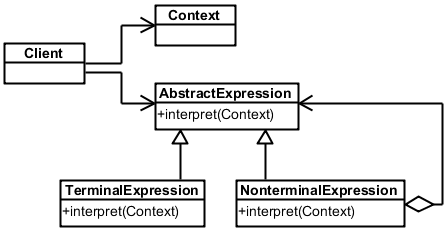
\includegraphics[width=0.6\textwidth]{interpreter.png}
        \end{center}
        \begin{itemize}
            \item Грамматика должна быть проста (иначе лучше ``Visitor'')
            \item Эффективность не критична
        \end{itemize}
    \end{frame}

    \begin{frame}
        \frametitle{``Интерпретатор'', пример}
        \begin{center}
            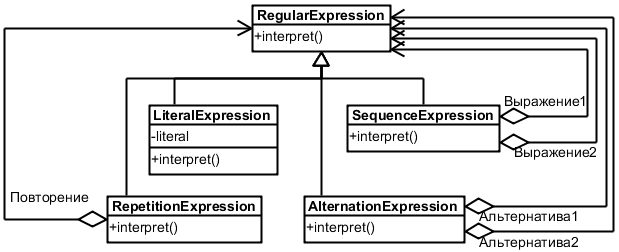
\includegraphics[width=0.8\textwidth]{regexp.png}
        \end{center}
    \end{frame}

    \begin{frame}
        \frametitle{``Интерпретатор'', детали реализации}
        \begin{footnotesize}
            \textbf{10-е правило Гринспена:}
            
            \textit{Любая достаточно сложная программа на Си или Фортране содержит заново написанную, неспецифицированную, глючную и медленную реализацию половины языка Common Lisp}
        \end{footnotesize}
        \begin{itemize}
            \item Построение дерева --- отдельная задача
            \item Несколько разных операций над деревом --- лучше ``Visitor''
            \item Можно использовать ``Приспособленец'' для разделения терминальных символов
        \end{itemize}
    \end{frame}

    \section{Паттерн ``Итератор''}

    \begin{frame}
        \frametitle{``Итератор'' (Iterator)}
        Инкапсулирует способ обхода коллекции.
        \begin{center}
            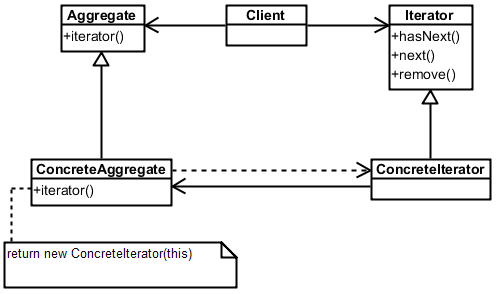
\includegraphics[width=0.6\textwidth]{iterator.png}
        \end{center}
        \begin{itemize}
            \item Разные итераторы для разных способов обхода
            \item Можно обходить не только коллекции
        \end{itemize}
    \end{frame}

    \begin{frame}[fragile]
        \frametitle{``Итератор'', примеры}
        \begin{itemize}
            \item Java-стиль:
            \begin{minted}{java}
public interface Iterator<E> {
    boolean hasNext();
    E next();
    void remove();
}
            \end{minted}
            \item .NET-стиль:
            \begin{minted}{csharp}
public interface IEnumerator<T>
{
    bool MoveNext();
    T Current { get; }
    void Reset();
}
            \end{minted}
        \end{itemize}
    \end{frame}

    \begin{frame}[fragile]
        \frametitle{``Итератор'', детали реализации (1)}
        \begin{itemize}
            \item Внешние итераторы
            \begin{minted}{csharp}
foreach (Thing t in collection)
{
    Console.WriteLine(t);
} 
            \end{minted}
            \item Внутренние итераторы
            \begin{minted}{csharp}
collection.ToList().ForEach(t => Console.WriteLine(t));
            \end{minted}
        \end{itemize}
    \end{frame}

    \begin{frame}
        \frametitle{``Итератор'', детали реализации (2)}
        \begin{itemize}
            \item Итераторы и курсоры
            \item Устойчивые и неустойчивые итераторы
            \begin{itemize}
                \item Паттерн ``Наблюдатель''
                \item Даже обнаружение модификации коллекции может быть непросто
            \end{itemize}
            \item Дополнительные операции
        \end{itemize}
    \end{frame}

\end{document}
